Our goal in this section is to break down the broad \texttt{MocaTree} to \texttt{Dictionary} transformation into smaller, modular steps. More specifically, we
want separate rules for transforming a \texttt{Folder} into its appropriate container element (i.e., \texttt{Library} or \texttt{Shelf}), then rules to
handle whatever \texttt{File} and \texttt{Node} elements they contain (such as transforming each of the \texttt{.dictionary} files into
\texttt{dictionary}, \texttt{author}, and \texttt{entry} elements).

\vspace{0.5cm}

\begin{figure}[htp]
\begin{center}
  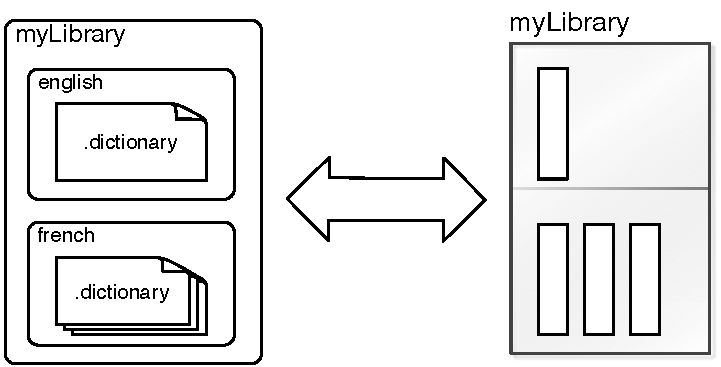
\includegraphics[width=0.7\textwidth]{treeToDictionaryTransformation}
  \caption{Transforming a \texttt{myLibrary} tree into an instance model}
  \label{fig:treeToDictionary}
\end{center}
\end{figure}

\vspace{0.5cm}

When creating \emph{any} rule, it's important to keep in mind any sort of flexibility the rule may require. In future \texttt{tree} instances for example, we
may not know how many exactly subfolders \texttt{myLibrary} will contain, whether or not each \texttt{.dictionary} file will have an author node (as seen in
\texttt{unknown.dictionary}), or how many entries each \texttt{dictionary} will contain. Just like SDMs, it's key to avoid situation-specific rules and
patterns.

\jumpDual{treeToModel vis}{treeToModel tex}
